\documentclass[a4paper,10pt]{article}
\usepackage[english]{babel}
\usepackage[utf8]{inputenc}
\usepackage{graphicx}
\usepackage{amsmath,amssymb}
\usepackage{hyperref, url}
\usepackage{listings}
\usepackage[multiple]{footmisc}
\usepackage[english]{babel}
\usepackage{float}
\parindent 0mm
\parskip 3mm

% add your name and student number in parenthesis
\title{ICS-E4020: Week 3 - Sorting/ImageSegmentation}
\author{Néstor Castillo García (472081)\\ 
       {\tt nestor.castillogarcia@aalto.fi}}
\begin{document}

\maketitle

\section{Parallel Merge Sort Algorithm}

\subsection{Description}

In this task a parallel version of merge sort was implemented. In the first step the data is divided into n parts and each thread sorts a single part. Then the parts are merged in parallel by pais until a single sorted chunk is obtained. The algorithm performs better if the number of threads is a power of two.


\subsection{Implementation}
The tests were made by sorting 100 million elements in cases large random integers, small random integers, constant input, increading values and decreasing values.


\subsection{Hardware}
The computers had the following specifications: Intel Xeon E3-1230v2, 4 cores, 8 thread, 3,3 GHz, RAM: 16 GB, GPU: Nvidia K2000.

\subsection{Performance}
As expected, performance increased with the number of threads. The multithreded version was in average 3,8 times faster than the single threaded solution for the large random case values. In the other cases there was a slight increase in speed.

\begin{figure}[H]
\centering
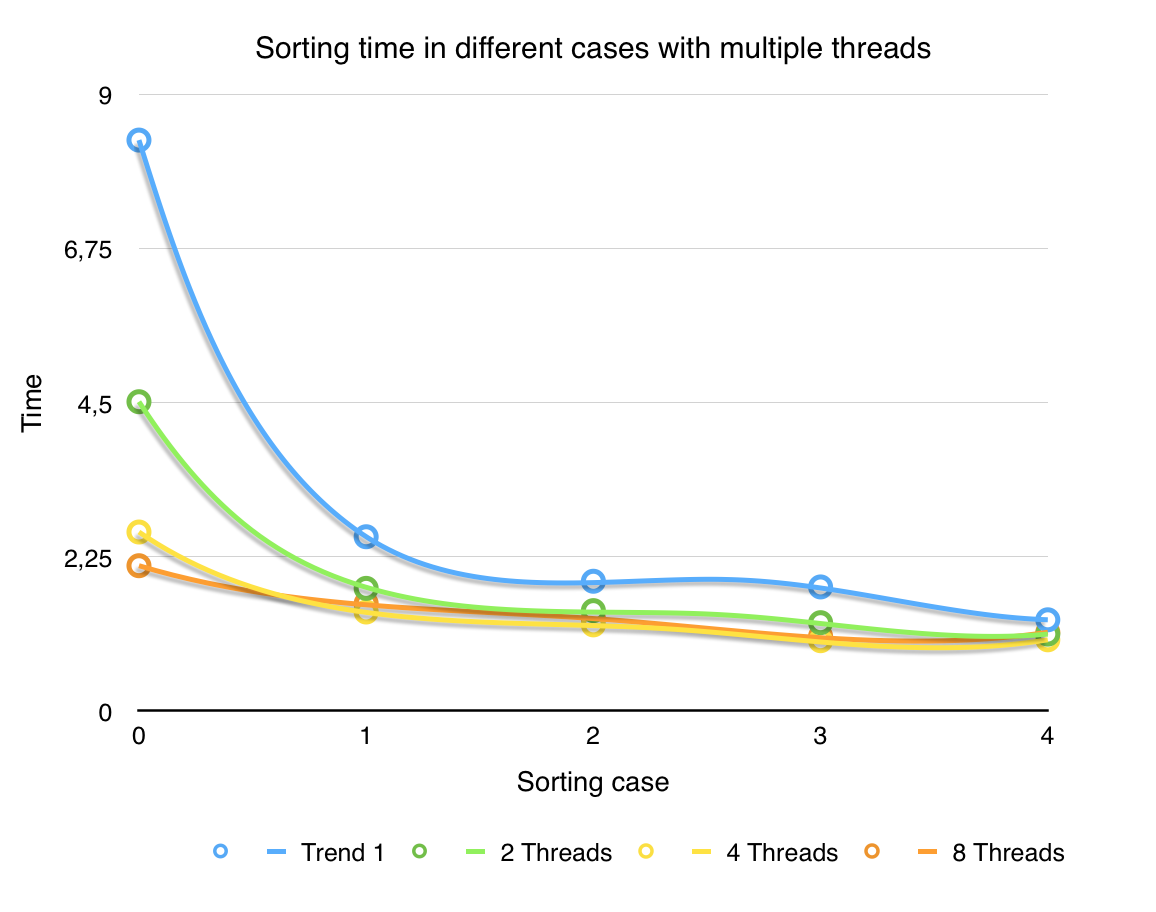
\includegraphics[width=1\textwidth]{figures/w3_SortingTime}
\caption{Multithreaded sorting time in cases:  0 = large random elements, 1 = small random elements, 2 = constant input, 3 = increasing values, and 4 = decreasing values.}
\label{fig:pca_type}
\end{figure}

NOTE: Resubmission CP2. I updated my cp2 file that was rejected because I misused malloc to free an array memory. 


I\end{document}